% Provenance (never printed): see sources/outline_sources.md (Year 3: Gibbs
% energy and the phase rule in rocks, chemical potential recalled from the
% chemistry book; ternary diagrams; pseudosections, principle). Brief:
% sources/book5/BRIEFS.md, ch. 11. Curves from figdata/bachelor-3/
% gasp_tables.py, schreinemakers.py and regular_solution.py. Exercise and
% problem values in the Book 5 scratch calculator calc/ch11.py.
\chapter{Termodinamika Batuan}\label{ch:b3:petrological-thermodynamics}

Sebuah garnet berdiameter beberapa milimeter tumbuh zona demi zona saat sekisnya terkubur
dan dipanaskan. Tepinya masih mencatat, dalam kalsium, besi, dan magnesiumnya,
kesetimbangan terakhir yang dicapainya dengan biotit dan plagioklas di sekelilingnya.
Volume Tahun 2 mengubah komposisi semacam itu menjadi suhu dan tekanan dengan
dua persamaan terkalibrasi. Bab ini membuka kotak itu: dari mana persamaan-persamaan itu berasal,
dan seberapa jauh tabel entalpi dan entropi terukur dapat
dipercaya, berapa banyak mineral yang dapat ditampung suatu batuan, bagaimana larutan padat bercampur dan
memisah, dan bagaimana komputer mengubah komposisi total menjadi peta
asosiasi mineral yang seharusnya ditampilkannya.

\begin{recall}
Energi Gibbs, potensial kimia, aktivitas, dan konstanta kesetimbangan,
varians dan aturan fasa, celah campur, dan aturan tuas
ada dalam volume universitas buku kimia. Reaksi univarian,
kemiringan Clapeyron $\Delta_rS/\Delta_rV$, titik invarian, dan
diagram aluminosilikat yang dihitung dari tabel ada dalam volume Tahun 2, pada babnya
tentang fasies metamorf; geotermometer dan geobarometer, serta
termometer pertukaran garnet--biotit dan barometer GASP, pada babnya tentang
lintasan P--T--t; diagram terner dan kotektik, pada babnya tentang magma. Sebuah
larutan padat dan anggota ujungnya ada dalam volume Tahun 1, pada babnya tentang
mineral.
\end{recall}

\section{Kesetimbangan dari tabel}\label{sec:b3:petrological-thermodynamics:tables}

Untuk reaksi di antara mineral dengan komposisi tetap, kesetimbangan pada
suhu $T$ dan tekanan $P$ adalah $\Delta_rG(T, P) = 0$. Tabel memberikan, pada
\qty{298.15}{K} dan \qty{1}{bar}, entalpi pembentukan, entropi, dan
volume molar setiap mineral, serta kapasitas kalor $C_p(T)$ di atas.
Volume Tahun 2 menganggap $\Delta_rH$, $\Delta_rS$ dan $\Delta_rV$ sebagai konstanta. Hasil
umumnya berikut ini.

\begin{theorem}[Energi Gibbs suatu reaksi pada $T$ dan $P$]\label{thm:b3:petrological-thermodynamics:dg}
Misalkan suatu reaksi memiliki, pada $T_0 = \qty{298.15}{K}$ dan \qty{1}{bar},
entalpi $\Delta_rH^\circ$ dan entropi $\Delta_rS^\circ$, serta kapasitas kalor
perubahan $\Delta_rC_p(T)$ dan, di antara padatan, perubahan volume $\Delta_rV$
yang tidak bergantung pada $T$ dan $P$. Maka
\[
  \Delta_rG(T, P) = \Delta_rH^\circ + \int_{T_0}^{T}\Delta_rC_p\,\mathrm dT
  - T\Bigl(\Delta_rS^\circ + \int_{T_0}^{T}\frac{\Delta_rC_p}{T}\,\mathrm dT\Bigr)
  + (P - 1)\,\Delta_rV ,
\]
dan garis kesetimbangannya adalah $P = 1 - \Delta_rG(T, 1)/\Delta_rV$.
\end{theorem}

\begin{proof}
Pada \qty{1}{bar}, $(\partial\Delta_rH/\partial T)_P = \Delta_rC_p$ dan
$(\partial\Delta_rS/\partial T)_P = \Delta_rC_p/T$; mengintegralkan dari $T_0$
menghasilkan $\Delta_rH(T)$ dan $\Delta_rS(T)$, serta $\Delta_rG = \Delta_rH -
T\Delta_rS$. Pada $T$ tetap, $(\partial\Delta_rG/\partial P)_T = \Delta_rV$,
konstan menurut hipotesis; mengintegralkan dari 1 ke $P$ menambahkan $(P - 1)\Delta_rV$.
Dengan menetapkan $\Delta_rG(T, P) = 0$ diperoleh garisnya.
\end{proof}

Kedua integral saling meniadakan sebagian: jumlahnya $\int_{T_0}^T\Delta_rC_p(1 -
T/T')\,\mathrm dT'$, dengan faktor $1 - T/T'$ yang bernilai negatif dan kecil
bila $T'$ dekat dengan $T$. Di antara padatan, $\Delta_rC_p$ sendiri kecil,
karena kapasitas kalor suatu mineral hampir sama dengan jumlah kapasitas kalor
oksidanya. Oleh karena itu, pendekatan sifat konstan cukup baik, dan
tabel menyatakan seberapa baik. Untuk reaksi GASP,
\[
  \ce{3 CaAl2Si2O8 <=> Ca3Al2Si3O12 + 2 Al2SiO5 + SiO2},
\]
tabel ringkasan memberikan $\Delta_rH^\circ = \qty{-36.3}{kJ}$,
$\Delta_rS^\circ = \qty{-130.7}{J.K^{-1}}$ dan $\Delta_rV =
\qty{-6.61}{J.bar^{-1}}$, sehingga garis berkemiringan \qty{19.8}{bar/K}. Tabel
suhu tinggi, yang memuat kapasitas kalor, memberikan
$\Delta_rG$ pada setiap \qty{100}{K}, dan kedua garis berbeda kurang dari
\qty{0.12}{kbar} hingga \qty{1200}{K} (gambar di bawah).
% ledger: rh95:gasp-298, rh95:gasp-ht

Eksperimen tidak sesuai sebaik itu. Dibalik dalam pres piston-silinder pada
900 hingga \qty{1250}{\celsius}, reaksi berada \qty{0.9}{kbar} lebih tinggi daripada
tabel pada \qty{627}{\celsius} dan \qty{1.9}{kbar} lebih tinggi pada
\qty{927}{\celsius}. Dengan $\Delta_rV = \qty{-6.61}{J.bar^{-1}}$,
\qty{1.9}{kbar} setara dengan galat \qty{12.6}{kJ} pada $\Delta_rH$; ketidakpastian
keempat entalpi pembentukan, \qty{3.2}{kJ} untuk
grosular, \qty{2.0}{kJ} untuk anortit dan kyanit, \qty{1.0}{kJ} untuk
kuarsa, bergabung menjadi sekitar \qty{8}{kJ} pada $\Delta_rH$. Kalorimetri menetapkan setiap
mineral hingga beberapa kilojoule; reaksi di antara unit rumus besar melipatgandakan
galat ini dan membaginya dengan perubahan volume yang kecil.
% ledger: rh95:gasp-298, kn88:gasp

\begin{definition}[Set data termodinamika yang konsisten secara internal]\label{def:b3:petrological-thermodynamics:dataset}
Sebuah \emph{set data termodinamika yang konsisten secara internal}\index{set data termodinamika yang konsisten secara internal}
adalah tabel sifat standar dari
banyak mineral dan fluida (entalpi pembentukan, entropi, volume, kapasitas kalor,
pemuaian termal, dan kompresibilitas) yang disesuaikan bersama, dalam batas
ketidakpastian kalorimetri, sehingga setiap kesetimbangan yang dihitung darinya
melewati eksperimen balik yang digunakan untuk mencocokkannya.
\end{definition}

Set data semacam itu dicocokkan sekali, dengan kuadrat terkecil berbobot atau
pemrograman linear terhadap semua batas eksperimen sekaligus, lalu dipakai untuk
setiap reaksi di antara mineralnya, termasuk reaksi yang belum pernah diteliti di
laboratorium. Angkanya bukan pengukuran independen: satu entalpi mungkin digeser
sebesar satu kilojoule agar cocok dengan reaksi yang ikut melibatkannya. Nilai dari
set data yang berbeda tidak boleh dicampur.

\begin{omfigure}
\begin{tikzpicture}
\begin{axis}[omrecord, width=0.78\linewidth, height=0.5\linewidth,
  xlabel={suhu (\unit{\celsius})}, ylabel={tekanan (\unit{kbar})},
  xmin=400, xmax=1300, ymin=0, ymax=30, legend style={font=\scriptsize,
  at={(0.03,0.97)}, anchor=north west, legend cell align=left}]
% computed in figdata/bachelor-3/gasp_tables.py
\fill[omLithLime!60] (axis cs:900,19) rectangle (axis cs:1250,28);
\addplot[red!70!black, very thick] table[x=tc, y=p_kn88] {figdata/out/bachelor-3-gasp_tables-lines.dat};
\addlegendentry{eksperimen (anggota ujung)}
\addplot[omDef, thick, densely dashed] table[x=tc, y=p_const] {figdata/out/bachelor-3-gasp_tables-lines.dat};
\addlegendentry{tabel, $\Delta_rH$, $\Delta_rS$ konstan}
\addplot[omDef, only marks, mark=*, mark size=1.8pt] table[x=tc, y=p_table] {figdata/out/bachelor-3-gasp_tables-tables.dat};
\addlegendentry{tabel, dengan kapasitas kalor}
\node[font=\scriptsize, align=center] at (axis cs:1075,26.3) {eksperimen\\balik};
\node[font=\scriptsize] at (axis cs:560,4) {anortit};
\node[font=\scriptsize, align=center] at (axis cs:560,17) {grosular + kyanit\\+ kuarsa};
\end{axis}
\end{tikzpicture}

\par\smallskip{\small Reaksi GASP anggota ujung, 3 anortit = grosular +
2 kyanit + kuarsa, dihitung dari tabel kalorimetrik dengan
sifat konstan (garis putus-putus) dan dengan kapasitas kalor (titik-titik), serta garis yang
dicocokkan pada eksperimen balik yang dilakukan di rentang berarsir (merah, diekstrapolasi di bawah
\qty{900}{\celsius}).}\label{fig:b3:petrological-thermodynamics:gasp}
\end{omfigure}
% ledger: rh95:gasp-298, rh95:gasp-ht, kn88:gasp

\section{Aturan fasa dalam batuan}\label{sec:b3:petrological-thermodynamics:phase-rule}

Aturan fasa kimia memberikan varians $F = c - p + 2$ bagi suatu sistem yang
terdiri atas $c$ komponen dalam $p$ fasa. Batuan termasuk sistem seperti ini, dan mineralnya
menunjukkan bagian bidang tekanan--suhu tempat batuan itu mencapai kesetimbangan.

\begin{proposition}[Aturan fasa mineralogi]\label{prop:b3:petrological-thermodynamics:goldschmidt}
Batuan yang telah mencapai kesetimbangan pada tekanan dan suhu yang dipilih
secara bebas dalam suatu area bidang tekanan--suhu memuat fasa tidak lebih banyak
daripada jumlah komponennya: $p \le c$. Inilah
\emph{aturan fasa mineralogi}\index{aturan fasa mineralogi}.
\end{proposition}

\begin{proof}
Aturan fasa memberikan $F = c - p + 2$ variabel intensif yang bebas. Jika
tekanan dan suhu keduanya dapat berubah tanpa mengubah asosiasi mineral, dua dari
variabel itu bebas: $F \ge 2$, sehingga $p \le c$. Batuan dengan $p = c + 1$ fasa
terletak pada garis univarian; dengan $p = c + 2$, pada titik invarian; keduanya
tidak mungkin pada batuan yang dipilih secara acak.
\end{proof}

Batuan yang melanggar aturan ini bisa saja telah mencapai kesetimbangan pada garis reaksi, yang
teksturnya mungkin memperlihatkan, atau tidak pernah mencapai kesetimbangan secara utuh: tekstur korona,
mineral berzonasi dan butir relik sering menjadi alasannya. Menghitung komponen
memerlukan kehati-hatian. Komponen yang hanya terdapat pada satu fasa dengan komposisi tetap, seperti
zirkon, dapat diabaikan bersama fasanya; komponen yang ditetapkan oleh reservoir eksternal,
seperti air ketika fluida mengalir melalui batuan, tidak dihitung
sebagai bebas, karena potensial kimianya sudah ditentukan dari luar.

Di sekitar titik invarian, garis univarian tidak berpotongan secara acak. Dalam
sistem dengan $c$ komponen, $c + 2$ fasa bertemu di titik itu, dan $c + 2$
reaksi memancar darinya, masing-masing ditulis di antara $c + 1$ fasa dan dinamai
menurut fasa yang dihilangkannya, dalam kurung.

\begin{definition}[Analisis Schreinemakers]\label{def:b3:petrological-thermodynamics:schreinemakers}
Yang disebut \emph{analisis Schreinemakers}\index{analisis Schreinemakers} ialah metode
yang menyusun garis univarian di sekitar titik invarian semata-mata dari
komposisi fasa-fasanya, sebelum pengukuran sifat termodinamikanya: ia menetapkan
urutan garis, sisi tiap garis yang stabil,
dan asosiasi mineral pada tiap sektor di antaranya.
\end{definition}

\begin{method}[Aturan Schreinemakers]\label{met:b3:petrological-thermodynamics:schreinemakers}
(1) Tulis $c + 2$ reaksi, masing-masing tanpa satu fasa. (2) Setiap garis
stabil di satu sisi titik dan metastabil di sisi lainnya. (3) Perpanjangan
metastabil garis ($i$), yang menghilangkan fasa $i$, terletak di sebuah
sektor tempat $i$ stabil. (4) Tidak ada sektor di antara dua garis stabil berurutan
yang merentang lebih dari \ang{180}. (5) Melintasi suatu garis, asosiasi di kedua sisinya
sesuai dengan kedua sisi reaksinya. Menetapkan satu garis dengan data kemudian
menetapkan seluruh berkas, kecuali bayangan cerminnya.
\end{method}

Titik tripel aluminosilikat dari volume Tahun 2 adalah kasus yang paling sederhana,
dengan $c = 1$ dan tiga garis. Gambar di bawah memperlihatkan kasus dua komponen
yang dihitung melalui \omterm{def:b3:petrological-thermodynamics:minimisation}{minimisasi energi Gibbs} di setiap titik.

\begin{omfigure}
\begin{tikzpicture}
\begin{axis}[omrecord, width=0.62\linewidth, height=0.5\linewidth,
  xlabel={suhu (\unit{\celsius})}, ylabel={tekanan (\unit{kbar})},
  xmin=400, xmax=800, ymin=1, ymax=9, grid=none]
% computed in figdata/bachelor-3/schreinemakers.py
\addplot[omDef, very thick] table[x=t, y=p] {figdata/out/bachelor-3-schreinemakers-ray_A_s.dat};
\addplot[omDef, thick, densely dashed] table[x=t, y=p] {figdata/out/bachelor-3-schreinemakers-ray_A_m.dat};
\addplot[omDef, very thick] table[x=t, y=p] {figdata/out/bachelor-3-schreinemakers-ray_B_s.dat};
\addplot[omDef, thick, densely dashed] table[x=t, y=p] {figdata/out/bachelor-3-schreinemakers-ray_B_m.dat};
\addplot[omDef, very thick] table[x=t, y=p] {figdata/out/bachelor-3-schreinemakers-ray_C_s.dat};
\addplot[omDef, thick, densely dashed] table[x=t, y=p] {figdata/out/bachelor-3-schreinemakers-ray_C_m.dat};
\addplot[omDef, very thick] table[x=t, y=p] {figdata/out/bachelor-3-schreinemakers-ray_D_s.dat};
\addplot[omDef, thick, densely dashed] table[x=t, y=p] {figdata/out/bachelor-3-schreinemakers-ray_D_m.dat};
\node[font=\scriptsize, fill=white, inner sep=1pt] at (axis cs:740,7.85) {(A)};
\node[font=\scriptsize, fill=white, inner sep=1pt] at (axis cs:540,8.75) {(C)};
\node[font=\scriptsize, fill=white, inner sep=1pt] at (axis cs:540,1.6) {(B)};
\node[font=\scriptsize, fill=white, inner sep=1pt] at (axis cs:740,2.15) {(D)};
\node[font=\scriptsize, align=center] at (axis cs:592,7.7) {A + B\\B + D};
\node[font=\scriptsize, align=center] at (axis cs:450,5.0) {A + D};
\node[font=\scriptsize, align=center] at (axis cs:592,2.4) {A + C\\C + D};
\node[font=\scriptsize, align=center] at (axis cs:765,5.0) {A + B\\B + C\\C + D};
\end{axis}
\end{tikzpicture}

\par\smallskip{\small Berkas Schreinemakers dalam sistem dua komponen dengan
empat fasa dengan komposisi A (0), B ($1/3$), C ($2/3$), dan D (1),
dihitung untuk sifat rekaan: garis stabil berupa garis penuh, perpanjangan metastabil
berupa garis putus-putus, serta pasangan stabil di tiap sektor. (D) adalah A + C = 2B, (A) adalah B + D =
2C, (C) adalah 2A + D = 3B dan (B) adalah A + 2D = 3C.}\label{fig:b3:petrological-thermodynamics:schreinemakers}
\end{omfigure}

\section{Larutan padat}\label{sec:b3:petrological-thermodynamics:solutions}

Sebagian besar mineral pembentuk batuan adalah larutan padat, dan anggota ujungnya
muncul dalam reaksi melalui aktivitasnya. Volume Tahun 2 mengambil $a = X^3$ untuk
grosular dalam garnet dan $a = X$ untuk anortit dalam plagioklas.
Keduanya merupakan kasus dari satu model.

\begin{definition}[Model aktivitas pencampuran situs]\label{def:b3:petrological-thermodynamics:site-mixing}
Dalam \emph{model aktivitas pencampuran situs}\index{model aktivitas pencampuran situs}, ion-ion
suatu mineral bercampur secara acak pada setiap situs kristalografi, secara bebas dari
situs lainnya. Aktivitas ideal suatu anggota ujung ialah hasil kali,
atas semua situs, dari fraksi setiap situs yang ditempatinya, dipangkatkan dengan jumlah
situs semacam itu per satuan rumus: $a_i = \prod_s X_{s,i}^{\,n_s}$.
\end{definition}

Garnet $X_3Y_2\ce{Si3O12}$ memiliki tiga situs dodekahedral $X$ untuk
\ce{Ca}, \ce{Fe}, \ce{Mg} dan \ce{Mn}: $a_{\text{grosular}} =
X_{\text{Ca}}^3$. Garnet dengan $X_{\text{Ca}} = 0.10$ mengandung
\qty{10}{\percent} grossular, tetapi aktivitasnya $10^{-3}$. Model ideal
menghitung konfigurasi; larutan nyata juga memiliki energi berlebih,
karena ion-ion berukuran berbeda menimbulkan regangan pada kisi.

\begin{definition}[Diagram energi Gibbs--komposisi]\label{def:b3:petrological-thermodynamics:gx}
Yang disebut \emph{diagram energi Gibbs--komposisi}\index{diagram energi Gibbs--komposisi}
memplot, pada suhu dan tekanan tetap, energi Gibbs molar setiap
fasa dalam suatu sistem terhadap komposisinya. Asemblase stabil dari komposisi total apa pun
terletak pada cembung bawah dari kurva-kurva tersebut: satu fasa
bila kurvanya berada pada cembung itu, dua fasa pada ujung-ujung garis singgung persekutuan.
\end{definition}

\begin{proposition}[Larutan reguler]\label{prop:b3:petrological-thermodynamics:regular}
Dalam larutan biner dengan satu situs pencampuran per satuan rumus dan
energi interaksi $W$, energi Gibbs pencampurannya ialah
\[
  G_{\text{mix}} = RT\bigl[x\ln x + (1 - x)\ln(1 - x)\bigr] + Wx(1 - x).
\]
Bila $W > 0$, larutan stabil pada setiap komposisi di atas $T_c =
W/(2R)$; di bawah $T_c$ kurvanya memiliki dua titik belok, dan komposisi
di antara kedua titik garis singgung persekutuannya terpisah menjadi dua fasa.
\end{proposition}

\begin{proof}
Suku pertama ialah $-T$ kali entropi konfigurasi pencampuran acak;
suku kedua, energi berlebih paling sederhana, simetris dan nol pada kedua ujung.
Dengan menurunkan dua kali, $G''_{\text{mix}} = RT/[x(1 - x)] - 2W$. Minimumnya
terhadap $x$ berada pada $x = 1/2$, di mana nilainya $4RT - 2W$, yang positif untuk
setiap $x$ bila $T > W/(2R)$. Di bawah itu, $G''_{\text{mix}} < 0$ pada suatu interval
di sekitar $1/2$: kurva melengkung ke bawah di sana, garis lurus di antara dua titik
kurva berada di bawahnya, dan menurut definisi di atas batuannya terdiri atas
dua fasa.
\end{proof}

\begin{definition}[Solvus, eksolusi]\label{def:b3:petrological-thermodynamics:solvus}
Yang disebut \emph{solvus}\index{solvus} ialah kurva, dalam bidang suhu--komposisi,
yang membatasi celah kelarutan campuran suatu larutan padat: di bawahnya, sebuah
kristal tunggal dengan komposisi antara tidak stabil dan terpecah menjadi dua.
Yang disebut \emph{eksolusi (mineral)}\index{eksolusi (mineral)} ialah pemecahan itu
di dalam satu kristal ketika mendingin: lamel dari satu komposisi tumbuh di dalam inang dari
komposisi lainnya.
\end{definition}

Feldspar alkali, piroksen dan amfibol menunjukkan lamel eksolusi,
yang tampak di bawah mikroskop atau dengan mata telanjang: perthit pada banyak granit
adalah feldspar alkali yang tereksolusi, dengan inang kaya kalium dan
lamel kaya natrium. Di antara \omterm{def:b3:petrological-thermodynamics:solvus}{solvus} dan spinodal, di tempat $G''_{\text{mix}} = 0$,
kristal harus lebih dulu menukleasi fasa kedua; di dalam spinodal, setiap
fluktuasi komposisi yang kecil tumbuh hanya oleh difusi.

\begin{omfigure}
\begin{tikzpicture}
\begin{groupplot}[group style={group size=2 by 1, horizontal sep=1.7cm},
  omrecord, width=0.47\linewidth, height=0.42\linewidth, title style={font=\small},
  legend style={font=\scriptsize, legend cell align=left}]
\nextgroupplot[title={(a) energi Gibbs pencampuran}, xlabel={$x$},
  ylabel={$G_{\text{mix}}$ (\unit{kJ.mol^{-1}})}, xmin=0, xmax=1, ymin=-9, ymax=1,
  legend style={at={(0.5,0.03)}, anchor=south}]
% computed in figdata/bachelor-3/regular_solution.py
\addplot[black, thick, densely dotted] table[x=x, y=g1500] {figdata/out/bachelor-3-regular_solution-gx.dat};
\addlegendentry{\qty{1500}{K}}
\addplot[red!70!black, thick, densely dashed] table[x=x, y=g1203] {figdata/out/bachelor-3-regular_solution-gx.dat};
\addlegendentry{$T_c = \qty{1203}{K}$}
\addplot[omDef, thick] table[x=x, y=g0900] {figdata/out/bachelor-3-regular_solution-gx.dat};
\addlegendentry{\qty{900}{K}}
\addplot[omDef, thin, forget plot] coordinates {(0.111,-0.635) (0.889,-0.635)};
\nextgroupplot[title={(b) solvus dan penampang pada $X_0 = 0.3$}, xlabel={$x$},
  ylabel={temperatur (\unit{K})}, xmin=0, xmax=1, ymin=600, ymax=1300,
  legend style={at={(0.5,0.03)}, anchor=south}]
\addplot[omDef, thick] table[x=x, y=t_bin] {figdata/out/bachelor-3-regular_solution-solvus.dat};
\addlegendentry{solvus}
\addplot[black, thick, densely dotted] table[x=x, y=t_spin] {figdata/out/bachelor-3-regular_solution-solvus.dat};
\addlegendentry{spinodal}
\addplot[red!70!black, thick, forget plot] coordinates {(0.3,600) (0.3,1300)};
\addplot[red!70!black, thick, densely dashed] table[x=x2, y=t] {figdata/out/bachelor-3-regular_solution-section.dat};
\addlegendentry{isoplet pada $X_0$}
\addplot[red!70!black, thick, densely dashed, forget plot] table[x=x1, y=t] {figdata/out/bachelor-3-regular_solution-section.dat};
\node[font=\scriptsize] at (axis cs:0.5,1250) {satu fasa};
\node[font=\scriptsize] at (axis cs:0.5,950) {dua fasa};
\end{groupplot}
\end{tikzpicture}

\par\smallskip{\small Larutan reguler dengan $W = \qty{20}{kJ.mol^{-1}}$
(ilustratif). (a) Energi Gibbs pencampuran pada tiga suhu; pada
\qty{900}{K} garis singgung persekutuan (garis tipis) menyentuh kurva di $x = 0.11$
dan 0.89. (b) \omterm{def:b3:petrological-thermodynamics:solvus}{Solvus} dan spinodal; batuan dengan komposisi total $X_0 =
0.3$ (garis merah vertikal) berupa satu fasa di atas \qty{1136}{K} dan dua fasa
di bawahnya, dengan komposisi yang mengikuti \omterm{def:b3:petrological-thermodynamics:solvus}{solvus} (putus-putus).}\label{fig:b3:petrological-thermodynamics:solvus}
\end{omfigure}

\section{Pseudoseksi}\label{sec:b3:petrological-thermodynamics:pseudosections}

Panel (b) pada gambar di atas sebenarnya sudah berupa \omterm{def:b3:petrological-thermodynamics:pseudosection}{pseudoseksi} kecil: untuk satu
komposisi total, ia menunjukkan fasa mana yang stabil pada setiap suhu, serta
komposisi dan proporsinya. Batuan metamorf memiliki sekitar sepuluh
komponen dan banyak larutan padat, tetapi prinsipnya sama.

\begin{definition}[Minimisasi energi Gibbs]\label{def:b3:petrological-thermodynamics:minimisation}
Yang disebut \emph{minimisasi energi Gibbs}\index{minimisasi energi Gibbs} mencari, pada suhu dan
tekanan tertentu, himpunan fasa, komposisinya, dan
jumlahnya yang meminimumkan energi Gibbs total suatu sistem dengan komposisi total
tetap, dengan syarat kekekalan setiap komponen.
\end{definition}

\begin{definition}[Pseudoseksi, isoplet, komposisi total efektif]\label{def:b3:petrological-thermodynamics:pseudosection}
Sebuah \emph{pseudoseksi}\index{pseudoseksi} ialah diagram fasa, biasanya pada bidang
tekanan--suhu, yang dihitung untuk satu komposisi total tetap: ia
terbagi atas medan-medan, masing-masing diberi label asemblase yang meminimumkan
energi Gibbs di situ. Sebuah \emph{isoplet (pseudoseksi)}\index{isoplet (pseudoseksi)}
ialah garis pada pseudoseksi, tempat suatu variabel komposisi
satu fasa, atau jumlahnya, bernilai konstan. Yang disebut \emph{komposisi total
efektif}\index{komposisi total efektif} ialah bagian dari komposisi batuan yang
masih ikut dalam kesetimbangan, setelah inti kristal berzonasi,
porfiroblas yang terisolasi dari matriks, dan bahan terisolasi lainnya
dibuang.
\end{definition}

\omterm{def:b3:petrological-thermodynamics:pseudosection}{Pseudoseksi} tidak menunjukkan garis univarian dalam arti
volume Tahun 2: pada sistem dengan larutan padat, batas antara dua medan
ialah tempat satu fasa muncul atau lenyap, dan posisinya bergantung pada
komposisi total. Membacanya langsung. Asemblase yang teramati menentukan sebuah medan;
komposisi mineral yang diukur, misalnya kalsium pada tepi garnet,
memilih satu isoplet di dalamnya; isoplet kedua, untuk unsur atau mineral lain,
atau mineral lain, memotongnya pada tekanan dan suhu
kesetimbangan. Garnet berzonasi memuat rangkaian perpotongan semacam itu, satu untuk tiap
zona, sepanjang lintasan batuan. Namun, ketika garnet tumbuh, intinya menyerap
mangan dan kalsium sehingga tak lagi terjangkau matriks: \omterm{def:b3:petrological-thermodynamics:pseudosection}{komposisi total efektif}
berubah, dan \omterm{def:b3:petrological-thermodynamics:pseudosection}{pseudoseksi} harus dihitung ulang untuk
zona yang lebih muda.

\begin{inthelab}[Meja petrolog]
\begin{minipage}[t]{0.55\linewidth}\vspace{0pt}
Petrolog mula-mula mengamati sayatan tipis di bawah mikroskop polarisasi,
untuk mengidentifikasi asemblase, teksturnya, dan butir-butir mana yang tumbuh
bersama-sama. Sayatan yang sama, setelah dilapisi karbon, kemudian dimasukkan ke mikroprob elektron
yang mengukur komposisi titik-titik berdiameter beberapa mikrometer
sepanjang profil melintasi garnet. Perangkat lunak yang meminimumkan energi Gibbs
dengan \omterm{def:b3:petrological-thermodynamics:dataset}{set data termodinamika yang konsisten secara internal} dan sejumlah model aktivitas menghitung
sebuah \omterm{def:b3:petrological-thermodynamics:pseudosection}{pseudoseksi} untuk komposisi total, yang diukur pada irisan batuan yang sama.
Isoplet dari komposisi terukur diplot di atasnya, dan titik perpotongannya
itulah jawabannya. Ketidakpastian set data dan model aktivitas,
bukan ketidakpastian pengukuran, biasanya yang membatasinya.
\end{minipage}\hfill
\begin{minipage}[t]{0.42\linewidth}\vspace{0pt}
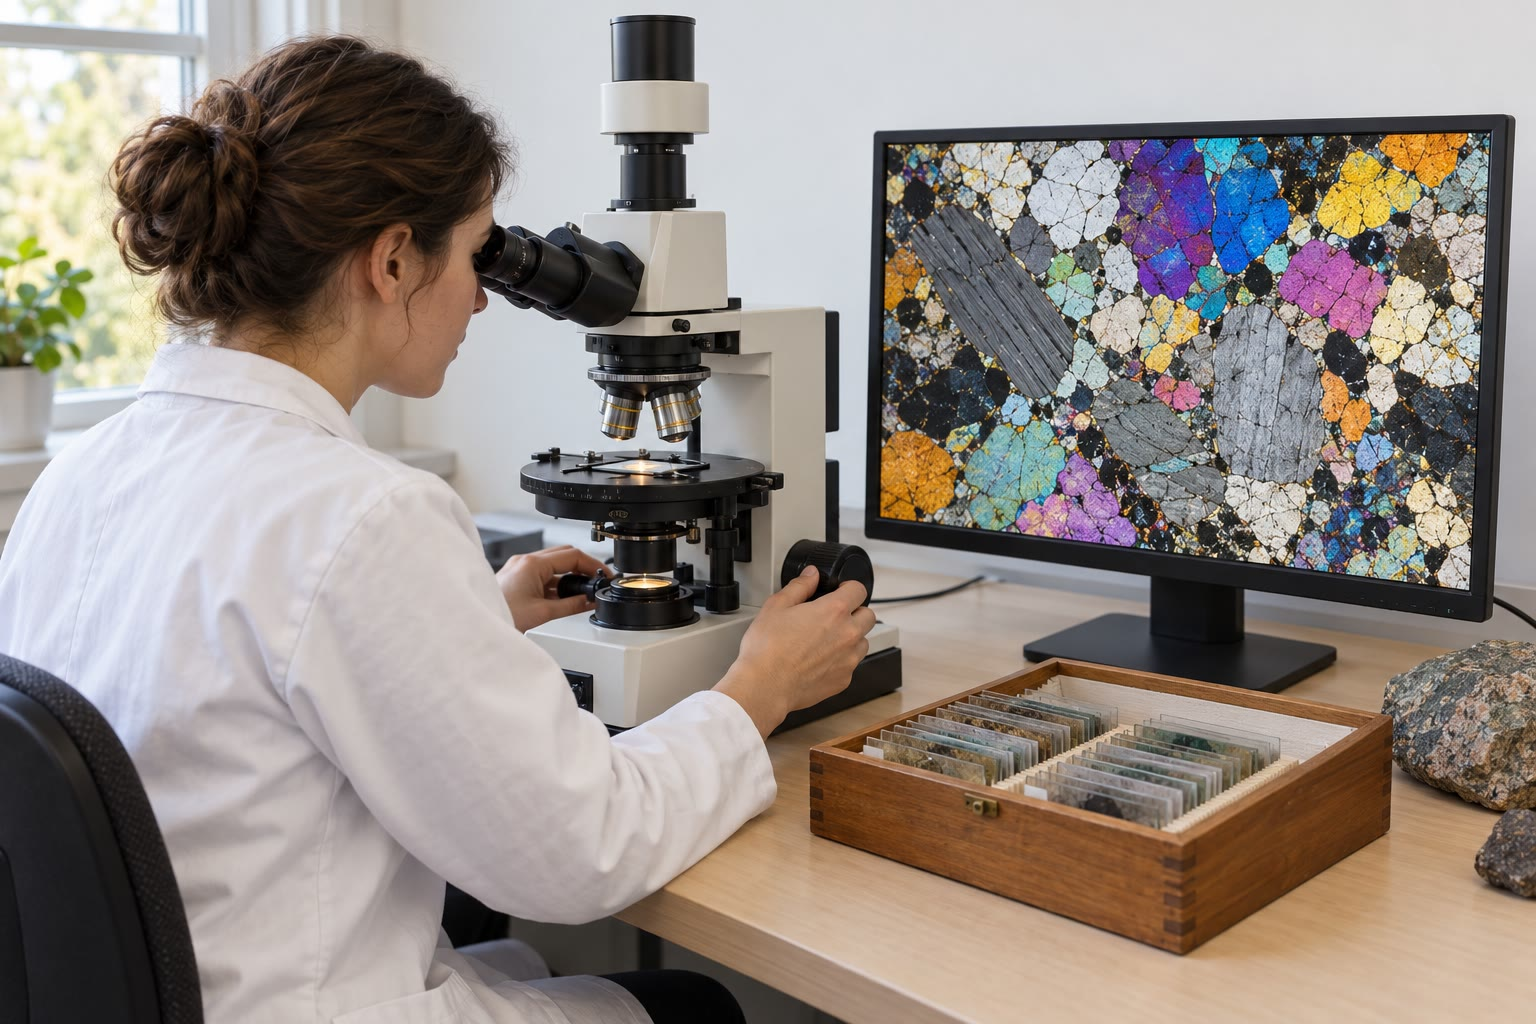
\includegraphics[width=\linewidth]{images/book5/ai/b3-petrology-desk.jpg}

{\scriptsize Seorang petrolog di depan mikroskop polarisasi, sekotak sayatan tipis
di dekatnya dan sebuah sayatan tipis dalam cahaya terpolarisasi di layar
(ilustrasi buatan AI).}
\end{minipage}
\end{inthelab}

\section{Latihan}

\begin{exercise}[$\star$]\label{exo:b3:petrological-thermodynamics:1}
Dari tabel, albit memiliki $\Delta_fH^\circ = \qty{-3935.0}{kJ}$, $S^\circ =
\qty{207.4}{J.K^{-1}}$, $V = \qty{100.07}{cm^3}$; jadeit $-3029.3$, 133.5,
60.40; kuarsa $-910.7$, 41.5, 22.69 (per mol). Untuk albit = jadeit + kuarsa,
hitung $\Delta_rH$, $\Delta_rS$, $\Delta_rV$ (dalam \unit{J.bar^{-1}}),
kemiringan Clapeyron dan tekanan garis pada \qty{600}{\celsius} dengan
sifat konstan.
\end{exercise}
% ledger: rh95:ab-jd-qz

\begin{exercise}[$\star$]\label{exo:b3:petrological-thermodynamics:2}
Sebuah batuan dalam sistem \ce{MgO}--\ce{SiO2} mengandung forsterit, enstatit dan
kuarsa. Terapkan \omterm{prop:b3:petrological-thermodynamics:goldschmidt}{aturan fasa mineralogi}. Apa kesimpulanmu?
\end{exercise}

\begin{exercise}[$\star$]\label{exo:b3:petrological-thermodynamics:3}
Hitung aktivitas ideal grosular dan pirop dalam garnet dengan
$X_{\text{Ca}} = 0.20$ dan $X_{\text{Mg}} = 0.15$, serta anortit dalam
plagioklas dengan $X_{\text{an}} = 0.40$ (satu situs).
\end{exercise}

\begin{exercise}[$\star$]\label{exo:b3:petrological-thermodynamics:4}
Hitung suhu kritis larutan reguler dengan $W =
\qty{15}{kJ.mol^{-1}}$. Berapa $W$ yang memberikan $T_c = \qty{1000}{K}$?
\end{exercise}

\begin{exercise}[$\star\star$]\label{exo:b3:petrological-thermodynamics:5}
Pada \qty{1000}{K}, tabel memberikan energi Gibbs pembentukan
$-5432.2$ (grosular), $-3478.1$ (anortit), $-2088.8$ (kyanit) dan $-730.2$
(kuarsa), dalam \unit{kJ.mol^{-1}}. Hitung $\Delta_rG$ reaksi GASP pada
\qty{1}{bar} dan tekanan kesetimbangannya, dan bandingkan dengan
garis eksperimen $P_0 = 22.80\,T - 1093$ (bar, \unit{\celsius}).
\end{exercise}
% ledger: rh95:gasp-ht, kn88:gasp

\begin{exercise}[$\star\star$]\label{exo:b3:petrological-thermodynamics:6}
Untuk larutan reguler pada gambar ($W = \qty{20}{kJ.mol^{-1}}$), hitung
$G_{\text{mix}}$ pada $x = 0.5$ dan \qty{900}{K}, lalu pada sayap \omterm{def:b3:petrological-thermodynamics:solvus}{solvus} $x =
0.111$. Tunjukkan bahwa membagi kristal dengan komposisi 0.5 menjadi dua sayap
menurunkan energi Gibbs-nya, dan berapa besarnya.
\end{exercise}

\begin{exercise}[$\star\star$]\label{exo:b3:petrological-thermodynamics:7}
Berapa fasa bertemu pada titik invarian, dan berapa garis univarian
memancar darinya, dalam sistem tiga komponen? Pada berkas dalam gambar,
periksa bahwa keempat reaksinya seimbang.
\end{exercise}

\begin{exercise}[$\star\star$]\label{exo:b3:petrological-thermodynamics:8}
Sebuah batuan dengan komposisi total $X_0 = 0.3$ dalam larutan reguler pada gambar
telah mendingin hingga \qty{900}{K}, ketika sayap \omterm{def:b3:petrological-thermodynamics:solvus}{solvusnya} berada pada 0.111 dan 0.889.
Hitung proporsi tiap fasa.
\end{exercise}

\begin{exercise}[$\star\star$]\label{exo:b3:petrological-thermodynamics:9}
Dengan barometer GASP $P = P_0 + (3RT/6.21)\ln(X_{\text{Ca}}/X_{\text{an}})$
(bar), hitung $\partial P/\partial X_{\text{an}}$ pada \qty{900}{K} dan
$X_{\text{an}} = 0.30$. Berapa besar galat 0.01 pada $X_{\text{an}}$
menggeser tekanan?
\end{exercise}

\begin{exercise}[$\star\star\star$]\label{exo:b3:petrological-thermodynamics:10}
Tunjukkan bahwa spinodal larutan reguler adalah $x(1 - x) = RT/(2W)$. Pada suhu berapa
kristal dengan komposisi 0.3 menjadi tidak stabil terhadap setiap fluktuasi kecil
untuk $W = \qty{20}{kJ.mol^{-1}}$? Bandingkan dengan suhu pada saat
kristal itu mencapai \omterm{def:b3:petrological-thermodynamics:solvus}{solvus}, $T = W(1 - 2x)/[R\ln((1 - x)/x)]$, dan jelaskan
selisih keduanya.
\end{exercise}

\begin{exercise}[$\star\star\star$]\label{exo:b3:petrological-thermodynamics:11}
Tunjukkan bahwa \omterm{def:b3:petrological-thermodynamics:solvus}{solvus} larutan reguler simetris memenuhi $RT\ln[x/(1 -
x)] + W(1 - 2x) = 0$, dan bahwa \omterm{def:b3:petrological-thermodynamics:solvus}{solvus} itu mencapai maksimum, $T_c = W/(2R)$, pada $x
= 1/2$.
\end{exercise}

\begin{exercise}[$\star\star\star$]\label{exo:b3:petrological-thermodynamics:12}
Batuan mengandung \qty{2.0}{wt\percent} \ce{MnO}. Inti garnet yang mengandung
\qty{10}{wt\percent} \ce{MnO} menyusun \qty{8}{wt\percent} batuan, dan
terisolasi dari matriks. Hitung kandungan \ce{MnO} dari \omterm{def:b3:petrological-thermodynamics:pseudosection}{komposisi total
efektif}. Mengapa hal itu penting bagi \omterm{def:b3:petrological-thermodynamics:pseudosection}{pseudoseksi} tepi garnet?
\end{exercise}

\section{Soal: Garnet pada sekis Varden}

\begin{problem}[{Soal akhir pekan --- tekanan dan suhu sekis rekaan,
dari tabel, aturan fasa, model aktivitas, dan
termobarometri}]
\label{pb:b3:petrological-thermodynamics:1}
% values: calc/ch11.py; gasp_tables.py
Sekis pada batuan dasar Bukit Varden, termetamorfosis sekitar
\qty{480}{Ma} lalu, mengandung garnet, biotit, muskovit, plagioklas, kianit dan
kuarsa. Pada tepi garnet dan butir di sekitarnya, mikroprob
memberikan: garnet $X_{\text{Fe}} = 0.74$, $X_{\text{Mg}} = 0.12$, $X_{\text{Ca}} =
0.10$, $X_{\text{Mn}} = 0.04$; biotit $\ce{Mg}/(\ce{Mg} + \ce{Fe}) = 0.45$;
plagioklas $X_{\text{an}} = 0.30$. Gunakan tabel bab ini untuk
reaksi GASP, termometer dari volume Tahun 2
\[
T = \frac{52\,635 + 0.311P}{20.20 - 3R\ln K_D}\quad(T \text{ dalam K}, P
\text{ dalam bar}),
\]
dan barometer eksperimennya $P = 22.80\,t - 1093 + (3RT/6.21)\ln
(X_{\text{Ca}}/X_{\text{an}})$, dengan $t$ dalam \unit{\celsius} dan $T$ dalam
kelvin. Ambil $R = \qty{8.314}{J.mol^{-1}.K^{-1}}$, massa jenis kerak sebesar
\qty{2800}{kg/m^3} dan $g = \qty{9.81}{m/s^2}$.

\medskip\noindent\textbf{Bagian I --- Tabel-tabel.}
\begin{enumerate}
  \item Dari tabel ringkasan, hitung $\Delta_rH^\circ$, $\Delta_rS^\circ$
        dan $\Delta_rV$ dari reaksi GASP.
  \item Hitung $\Delta_rG$ pada \qty{298.15}{K} dan \qty{1}{bar}. Sisi mana
        yang stabil di permukaan?
  \item Hitung tekanan anggota ujung pada \qty{900}{K} dengan sifat konstan,
        dan kemiringan Clapeyron.
  \item Tabel suhu tinggi memberikan $\Delta_rG = \qty{81.5}{kJ}$ pada
        \qty{900}{K} dan \qty{119.8}{kJ} pada \qty{1200}{K} (\qty{1}{bar}).
        Hitung tekanan-tekanannya.
  \item Bandingkan dengan garis eksperimen pada suhu yang sama.
  \item Kesalahan apa pada $\Delta_rH$ yang dapat menjelaskan celah pada \qty{1200}{K}?
        Bandingkan dengan ketidakpastian gabungan dari keempat entalpi.
  \item Mengapa kapasitas panas hanya sedikit mengubah hasilnya?
\end{enumerate}

\medskip\noindent\textbf{Bagian II --- Aturan fasa.}
\begin{enumerate}[resume]
  \item Daftarkan komponen yang diperlukan untuk mendeskripsikan keenam mineral dan
        fluida air, lalu hitung fasanya.
  \item Hitung varians dengan aturan fasa, dan periksa \omterm{prop:b3:petrological-thermodynamics:goldschmidt}{aturan
        fasa mineralogi}.
  \item Sampel kedua mengandung kianit dan silimanit berdampingan. Apa yang
        hal itu katakan tentang tekanan dan suhunya?
  \item Air mengalir melalui batuan selama metamorfisme. Bagaimana hal itu
        mengubah hitungannya?
\end{enumerate}

\medskip\noindent\textbf{Bagian III --- Aktivitas dan termobarometri.}
\begin{enumerate}[resume]
  \item Hitung aktivitas ideal grossular dan anortit, serta $\ln K$
        reaksi GASP dalam batuan.
  \item Hitung $K_D$ pertukaran garnet--biotit.
  \item Hitung suhu pada \qty{8}{kbar}.
  \item Hitung tekanan GASP pada suhu tersebut.
  \item Iterasikan hingga perpotongan kedua persamaan.
  \item Ulangi perpotongan dengan garis anggota ujung dari tabel sebagai pengganti
        garis eksperimen (dengan $\Delta_rV = \qty{-6.61}{J.bar^{-1}}$).
        Hasil mana yang kamu pertahankan, dan mengapa?
  \item Seberapa besar kesalahan 0.05 pada $X_{\text{an}}$ menggeser
        hasilnya?
\end{enumerate}

\medskip\noindent\textbf{Bagian IV --- Penguburan.}
\begin{enumerate}[resume]
  \item Dengan sifat konstan dari volume Tahun 2, kianit =
        silimanit memiliki $\Delta_rH = \qty{7.7}{kJ}$, $\Delta_rS =
        \qty{12.6}{J.K^{-1}}$, $\Delta_rV = \qty{0.571}{J.bar^{-1}}$. Apakah
        hasilnya berada di medan kianit?
  \item Hitung kedalaman penguburan.
  \item Inti garnet memiliki $X_{\text{Ca}} = 0.07$ dan tumbuh bersama plagioklas
        dengan $X_{\text{an}}$ yang sama, pada suhu yang kurang lebih sama. Apakah
        inti itu terbentuk lebih dalam atau lebih dangkal daripada tepinya?
  \item Berikan tekanan puncak dan kedalaman penguburan sekis Varden.
\end{enumerate}
\end{problem}
